\pdfoutput=1

\documentclass[11pt]{article}

\usepackage[guidelines]{nlpreport}
\usepackage{times}
\usepackage{latexsym}
\usepackage{verbatim}
\usepackage[T1]{fontenc}
\usepackage[utf8]{inputenc}
\usepackage{microtype}
\usepackage{graphicx}
\usepackage{hyperref}
\usepackage{amsmath}
\usepackage{mathtools}
\usepackage{multirow}
\usepackage{listings}
\usepackage{xcolor}
\usepackage{booktabs}
\hypersetup{pdfinfo={
Title={Assignment 1: Part-Of-Speech Tagging},
Author={Mattia Maranzana \& Antonios Pantelis \& Nalin Sharma}
}}
%\setcounter{secnumdepth}{0}  
\begin{document}

\title{Assignment 1: Part of Speech Tagging on the Penn Treebank Tagset}

\author{Mattia Maranzana,
Antonios Pantelis,
\and
Nalin Sharma\\
Master's Degree in Artificial Intelligence, University of Bologna\\
\{mattia.maranzana, antonios.pantelis, nalin.sharma\}@studio.unibo.it
}
\maketitle

\begin{abstract}
%\begin{quote}
In this project we are called to address the classification task of Part of Speech (POS) Tagging on the pre-tagged Penn Treebank Tagset. Our goal is to elevate accuracy, leveraging the text pre-processing and NLP model development techniques that we explored in the course and during Tutorials 1 and 2.
%\end{quote}
\end{abstract}

\section{Introduction}

As we mentioned previously, we are addressing the supervised learning task of POS tagging on the Penn Treebank dataset. Let us give a brief summary of our approach.

We encoded the Tagset into two \texttt{pandas} dataframes, namely \texttt{df} (corpus split by sentences) and \texttt{df\_file} (corpus split by file), for further analysis. We then split both dataframes into training, validation, and test sets, adding an additional "split" column to identify each piece of data with its corresponding dataset.

Then, we performed basic data inspection, visualizations, and text pre-processing, as detailed in section "\nameref{sec:data}."

Furthermore, we built the vocabulary of the corpus, along with \texttt{idx\_to\_word} and \texttt{word\_to\_idx} maps, and conducted tokenization.

Next up, we downloaded GloVe embeddings and calculated the percentage of Out of Vocabulary (OOV) words. For the validation and test sets, we addressed OOV words by replacing them with token "UNK". The subsequent creation of an embedding matrix involved using GloVe embeddings for known words, zero vectors for "UNK", and random vectors for remaining OOV words. Moreover, padding was applied at the beginning of each sequence, and sentences exceeding a length of 600 were truncated.

Following this, we performed some data preparation that included One-Hot Encoding, and size verification.

Later on, we created a variable, \texttt{punctuation\_indices}, to store punctuation indices for later exclusion during metric evaluation, developed a macro multi-class $F_1$ score metric and proceeded to create the three models.

Finally, after training our models, we conducted basic error analysis by identifying misclassified tags and their corresponding words to explore potential correlations.


\section{System description}
\label{sec:system}

For the creation of our models, we used the \texttt{Keras}\footnote{This was precisey the reason why we had to define the metric $F_1$ ourselves, since the already defined one of \texttt{scikit-learn} is incompatible with \texttt{Tensorflow}.} library of \texttt{Tensorflow}. As instructed, we developed three models, whose architectures can be seen in Figure \ref{fig:Models}.

\begin{figure*}
    \begin{minipage}{.3\textwidth}
      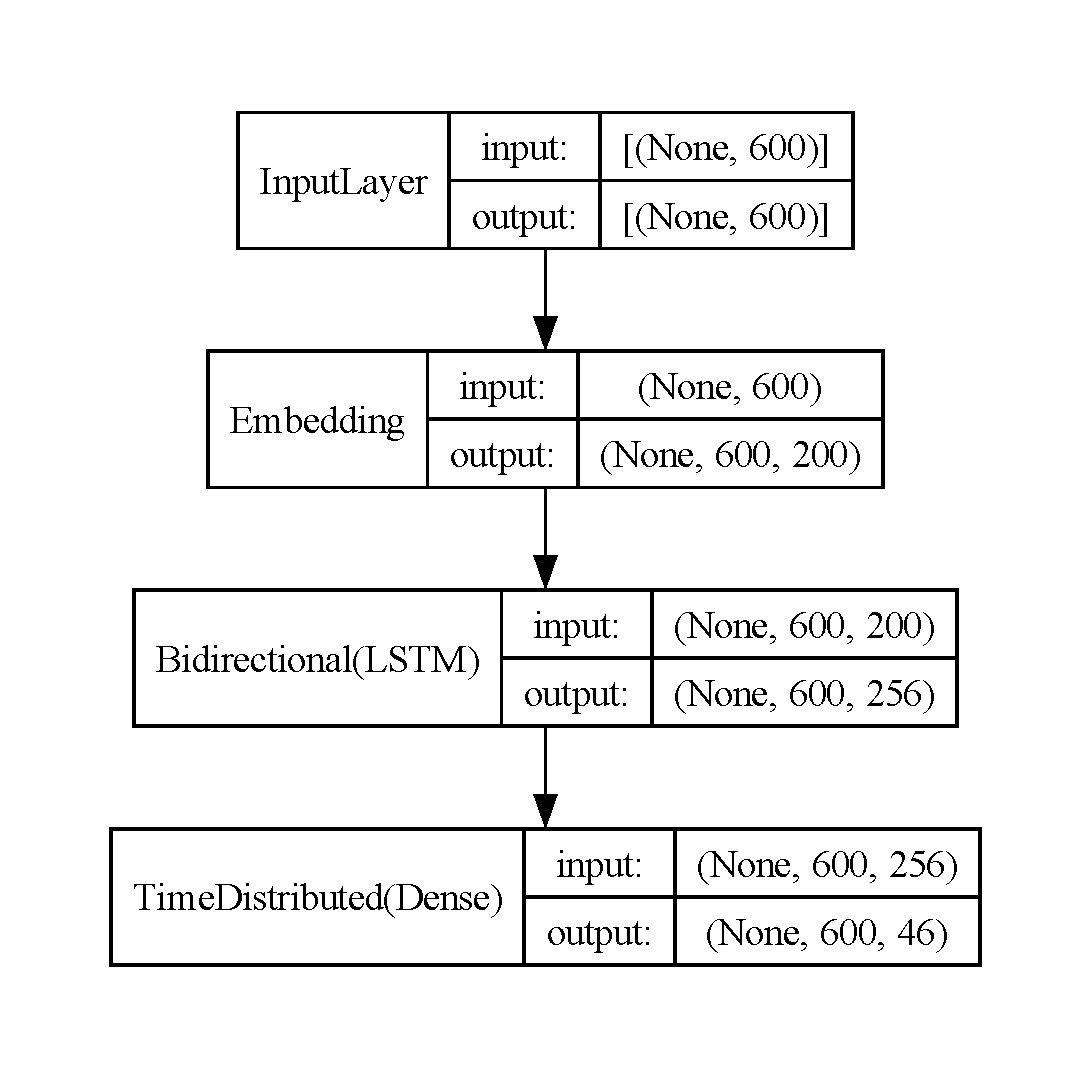
\includegraphics[width=\linewidth]{baseline_model.pdf}
      %\caption{Baseline Model}
      %\label{fig:baseline}
    \end{minipage} \quad
    \begin{minipage}{.3\textwidth}
      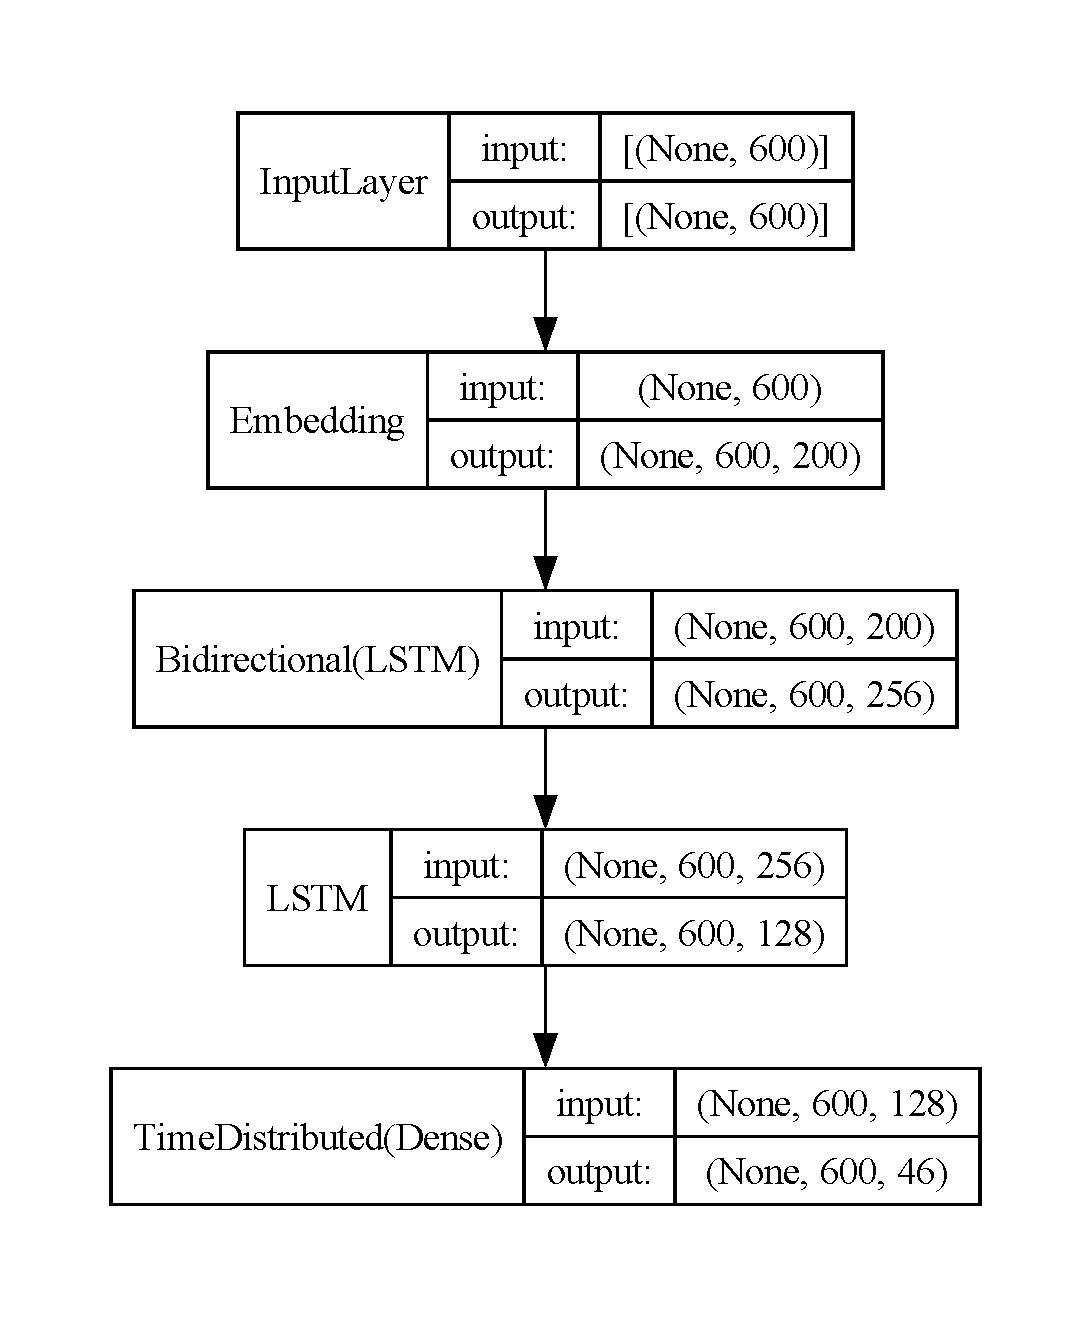
\includegraphics[width=\linewidth]{model_1.pdf}
      %\caption{Model 1}
      %\label{fig:model1}
    \end{minipage} \quad
    \begin{minipage}{.3\textwidth}
      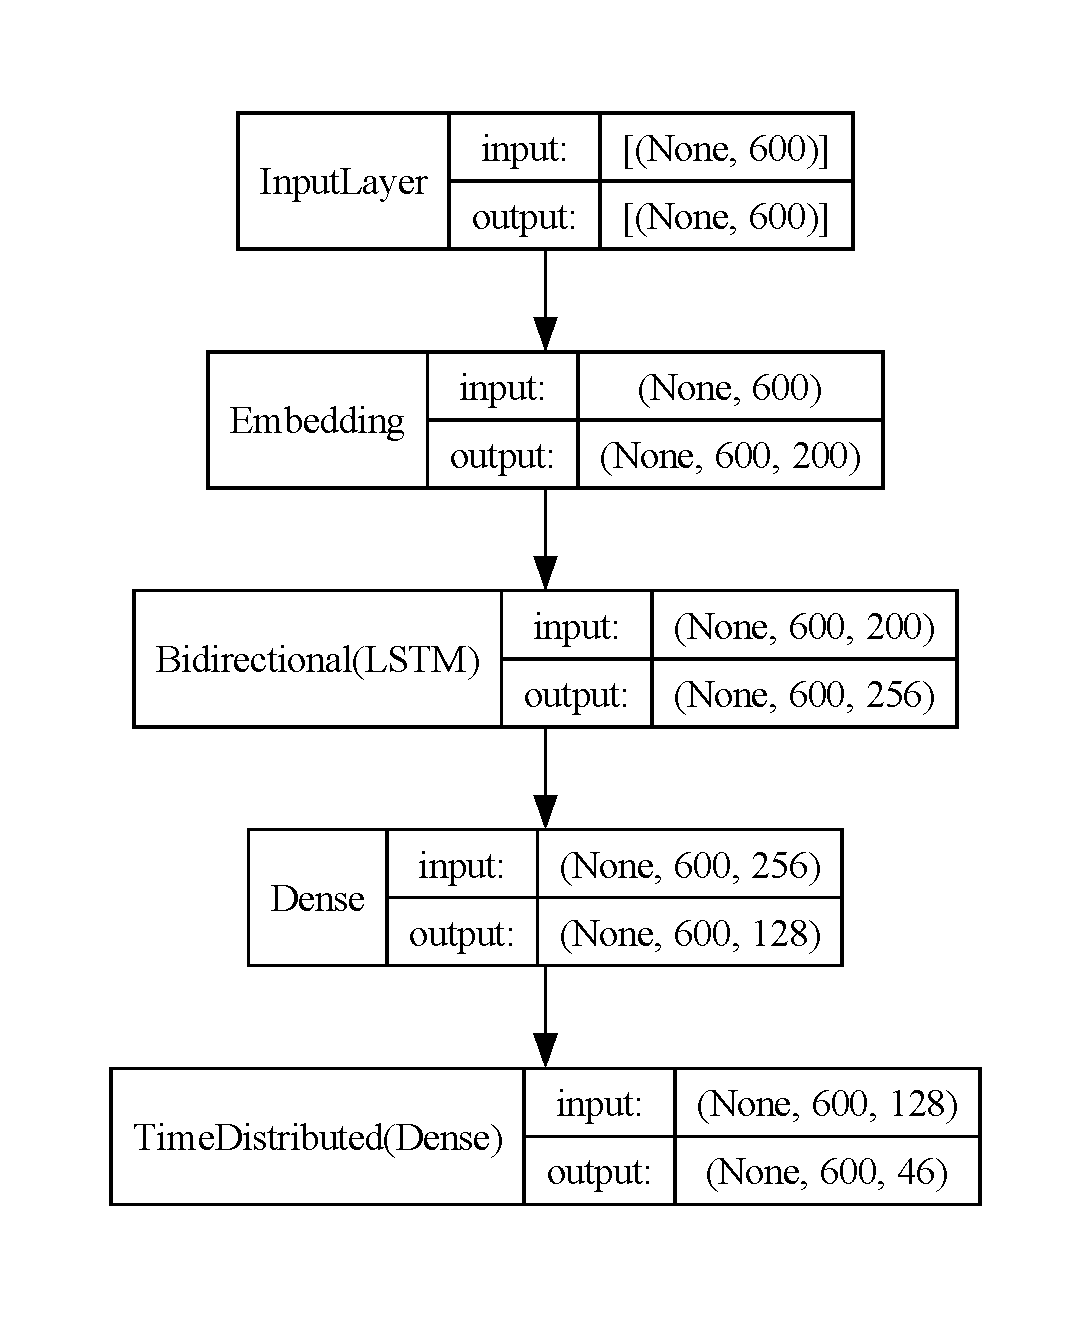
\includegraphics[width=\linewidth]{model_2.pdf}
      %\caption{Model 2}
      %\label{fig:model2}
    \end{minipage}
    \caption{Architectures of \texttt{baseline\_model} (left), \texttt{model\_1} (center), and \texttt{model\_2} (right).}
    \label{fig:Models}
\end{figure*}

\section{Data}
\label{sec:data}
As far as data inspection goes, we calculated the distribution of individual words in sentences and the distribution of POS tags and plotted the 20 \emph{most}\footnote{Most of the \emph{most frequent} words included punctuation and stop words.} and \emph{least frequent}\footnote{Some of the \emph{least frequent} words included numbers and names.} words. 

Furthermore, we created a dictionary for the POS labels and performed some minimal text pre-processing on the corpus. In particular, we chose to simply make every word in the corpus lower case, since we could not delete or modify any tokens. This helped greatly with the OOV words percentage. In particular, we obtained $4.98\%$ after lower-casing, while before we had obtained approximately $20\%$. This made the OOV percentage negligible and thus we decided that no further handling of the OOV words was required.

Moreover, we also plotted two box plots showing the distribution of sentences' lengths. This helped us make an informed decision about the padding. Since the beginning of the project we had two ideas in mind: either truncate sequences at a fixed padding length with the risk of losing some information, or trying to divide each file in sub-sentences of fixed length and pad them accordingly as not to lose any information at all. However, from the two box plots in question, it was clear that the more convenient one is that of truncating each sentence at length equal to 600. With this choice, we lose only a negligible amount of information out of only one sentence whose length is as one can see from both box plots around twice the padding length.

\section{Experimental setup and results}
\label{sec:results}
For the remaining hyperparameters, that is embedding dimension, batch size, learning rate and trainability, we performed three different grid searches, for each model and respectively set them to 200, 128, 0.01 and True. Finally, for the \emph{units}\footnote{This hyperparameter was also included in the grid search.} in both the bidirectional LSTM layer and the LSTM layer of \texttt{model\_2} we set it to 128.

% TODO: Add tables with results (all models?)


\section{Discussion}
\label{sec:discussion}
\attention{MAX 1.5 COLUMNS FOR ASSIGNMENT REPORTS / 3 COLUMNS FOR PROJECT / 4 FOR COMBINED REPORTS. ADDITIONAL EXAMPLES COULD BE PLACED IN AN APPENDIX AFTER THE REFERENCES IF THEY DO NOT FIT HERE.}


\explanation{
Here you should make your analysis of the results you obtained in your experiments. Your discussion should be structured in two parts: 
\begin{itemize}
    \item discussion of quantitative results (based on the metrics you have identified earlier; compare with baselines);
    \item error analysis: show some examples of odd/wrong/unwanted  outputs; reason about why you are getting those results, elaborate on what could/should be changed in future developments of this work.
\end{itemize}
}



\section{Conclusion}
\label{sec:conclusion}
\attention{MAX 1 COLUMN.}

\explanation{
In one or two paragraphs, recap your work and main results.
What did you observe? 
Did all go according to expectations? 
Was there anything surprising or worthwhile mentioning?
After that, discuss the main limitations of the solution you have implemented, and indicate promising directions for future improvement.
}

\end{document}